\section{Веб-приложение}\label{sec:-2}

\subsection{Аутентификация}\label{subsec:}
Стартовая страница.
На ней происходит аутентификация врача и пациента.
Так же можно перейти на страницу регистрации врача
\begin{figure}[h]
    \centering
    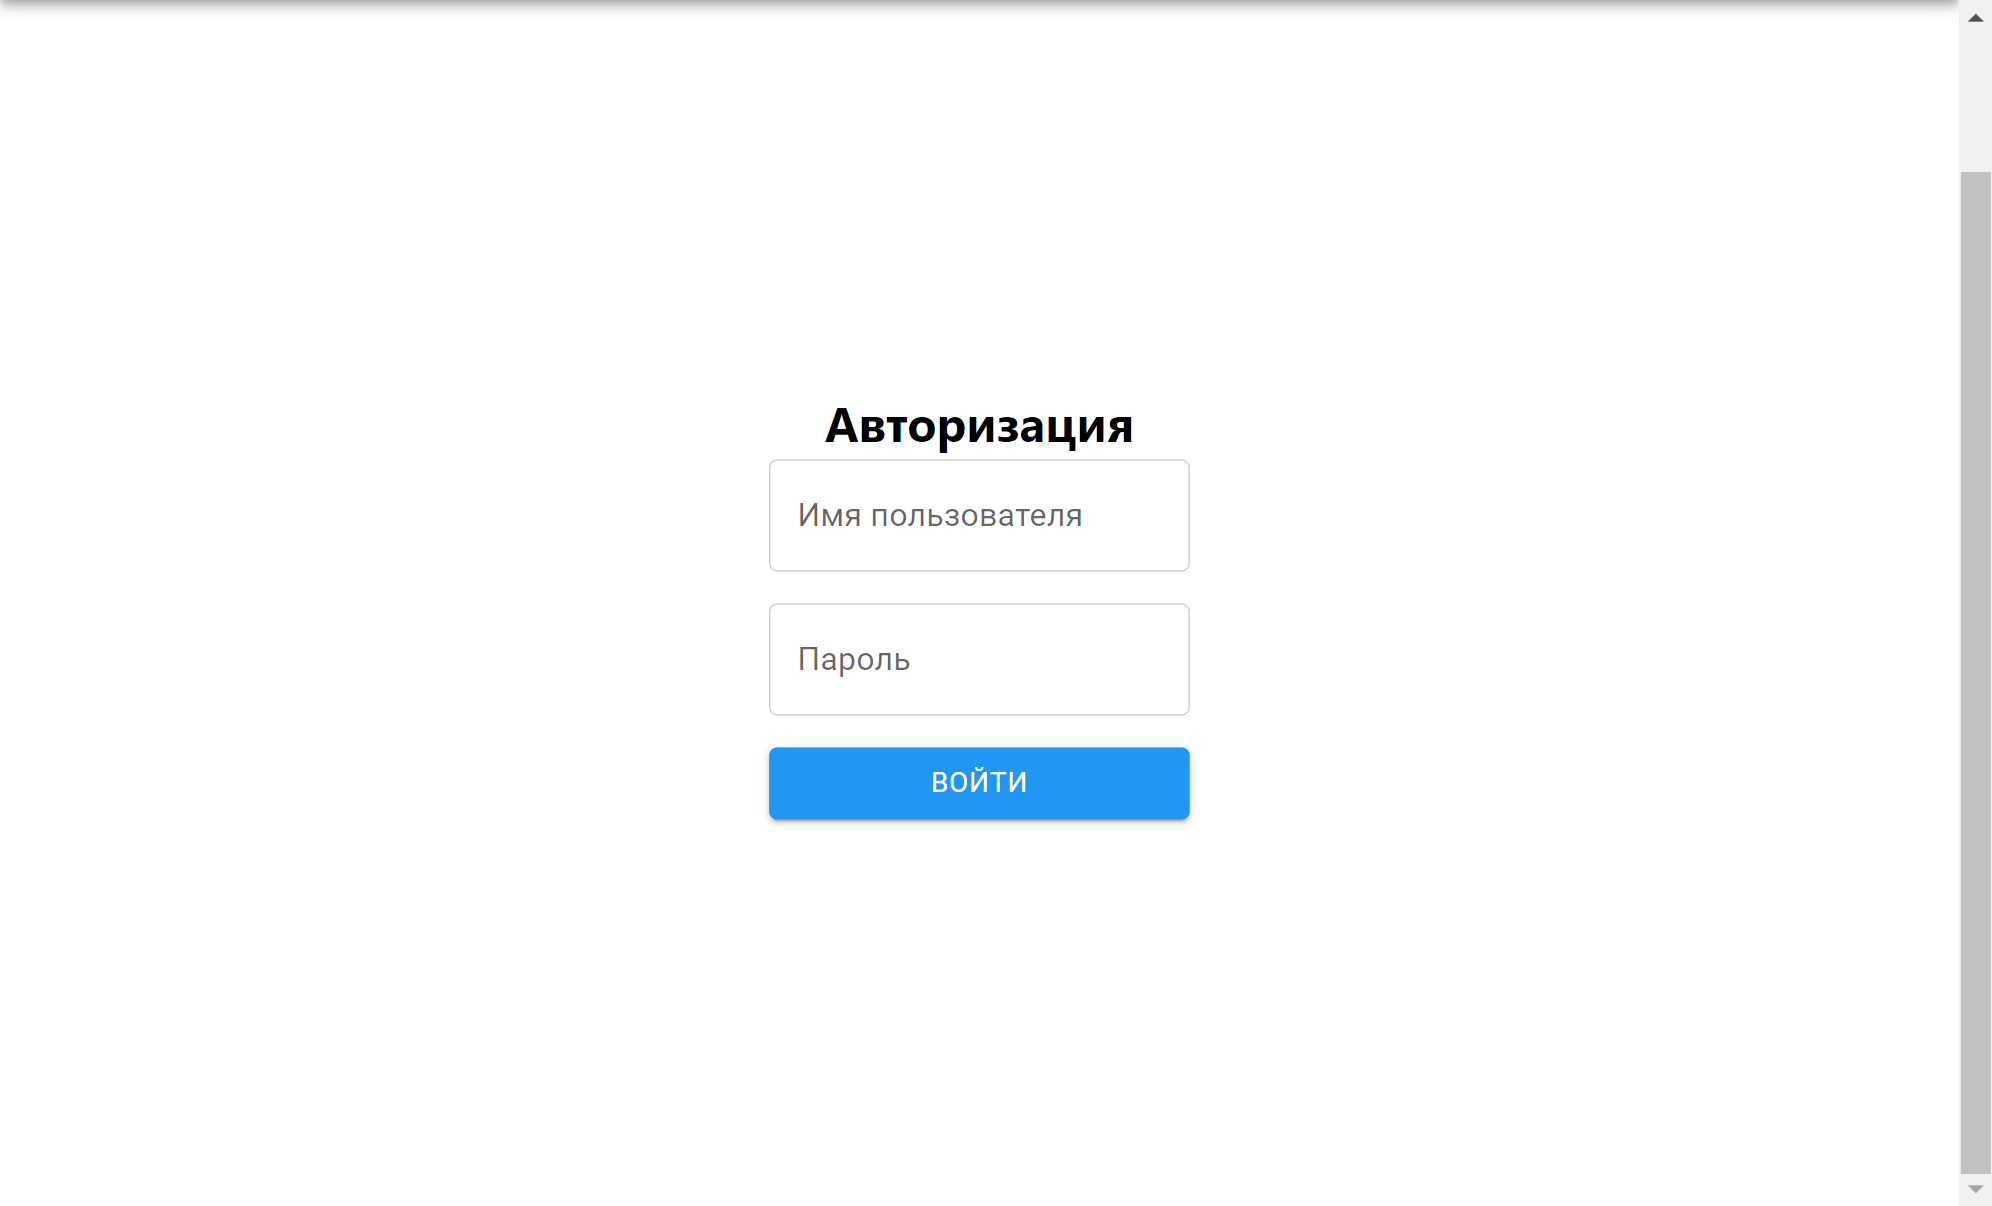
\includegraphics[width=\textwidth]{images/screenshots/auth}
    \caption{Аутентификация.}
    \label{fig:figure4}
\end{figure}


\subsection{Регистрация врача}\label{subsec:-5}
Здесь при первом посещении портала врач может авторизоваться.
(См.\ рис. \ref{fig:figure41})
При успешной авторизации врач сразу авторизуется
\begin{figure}[h]
    \centering
    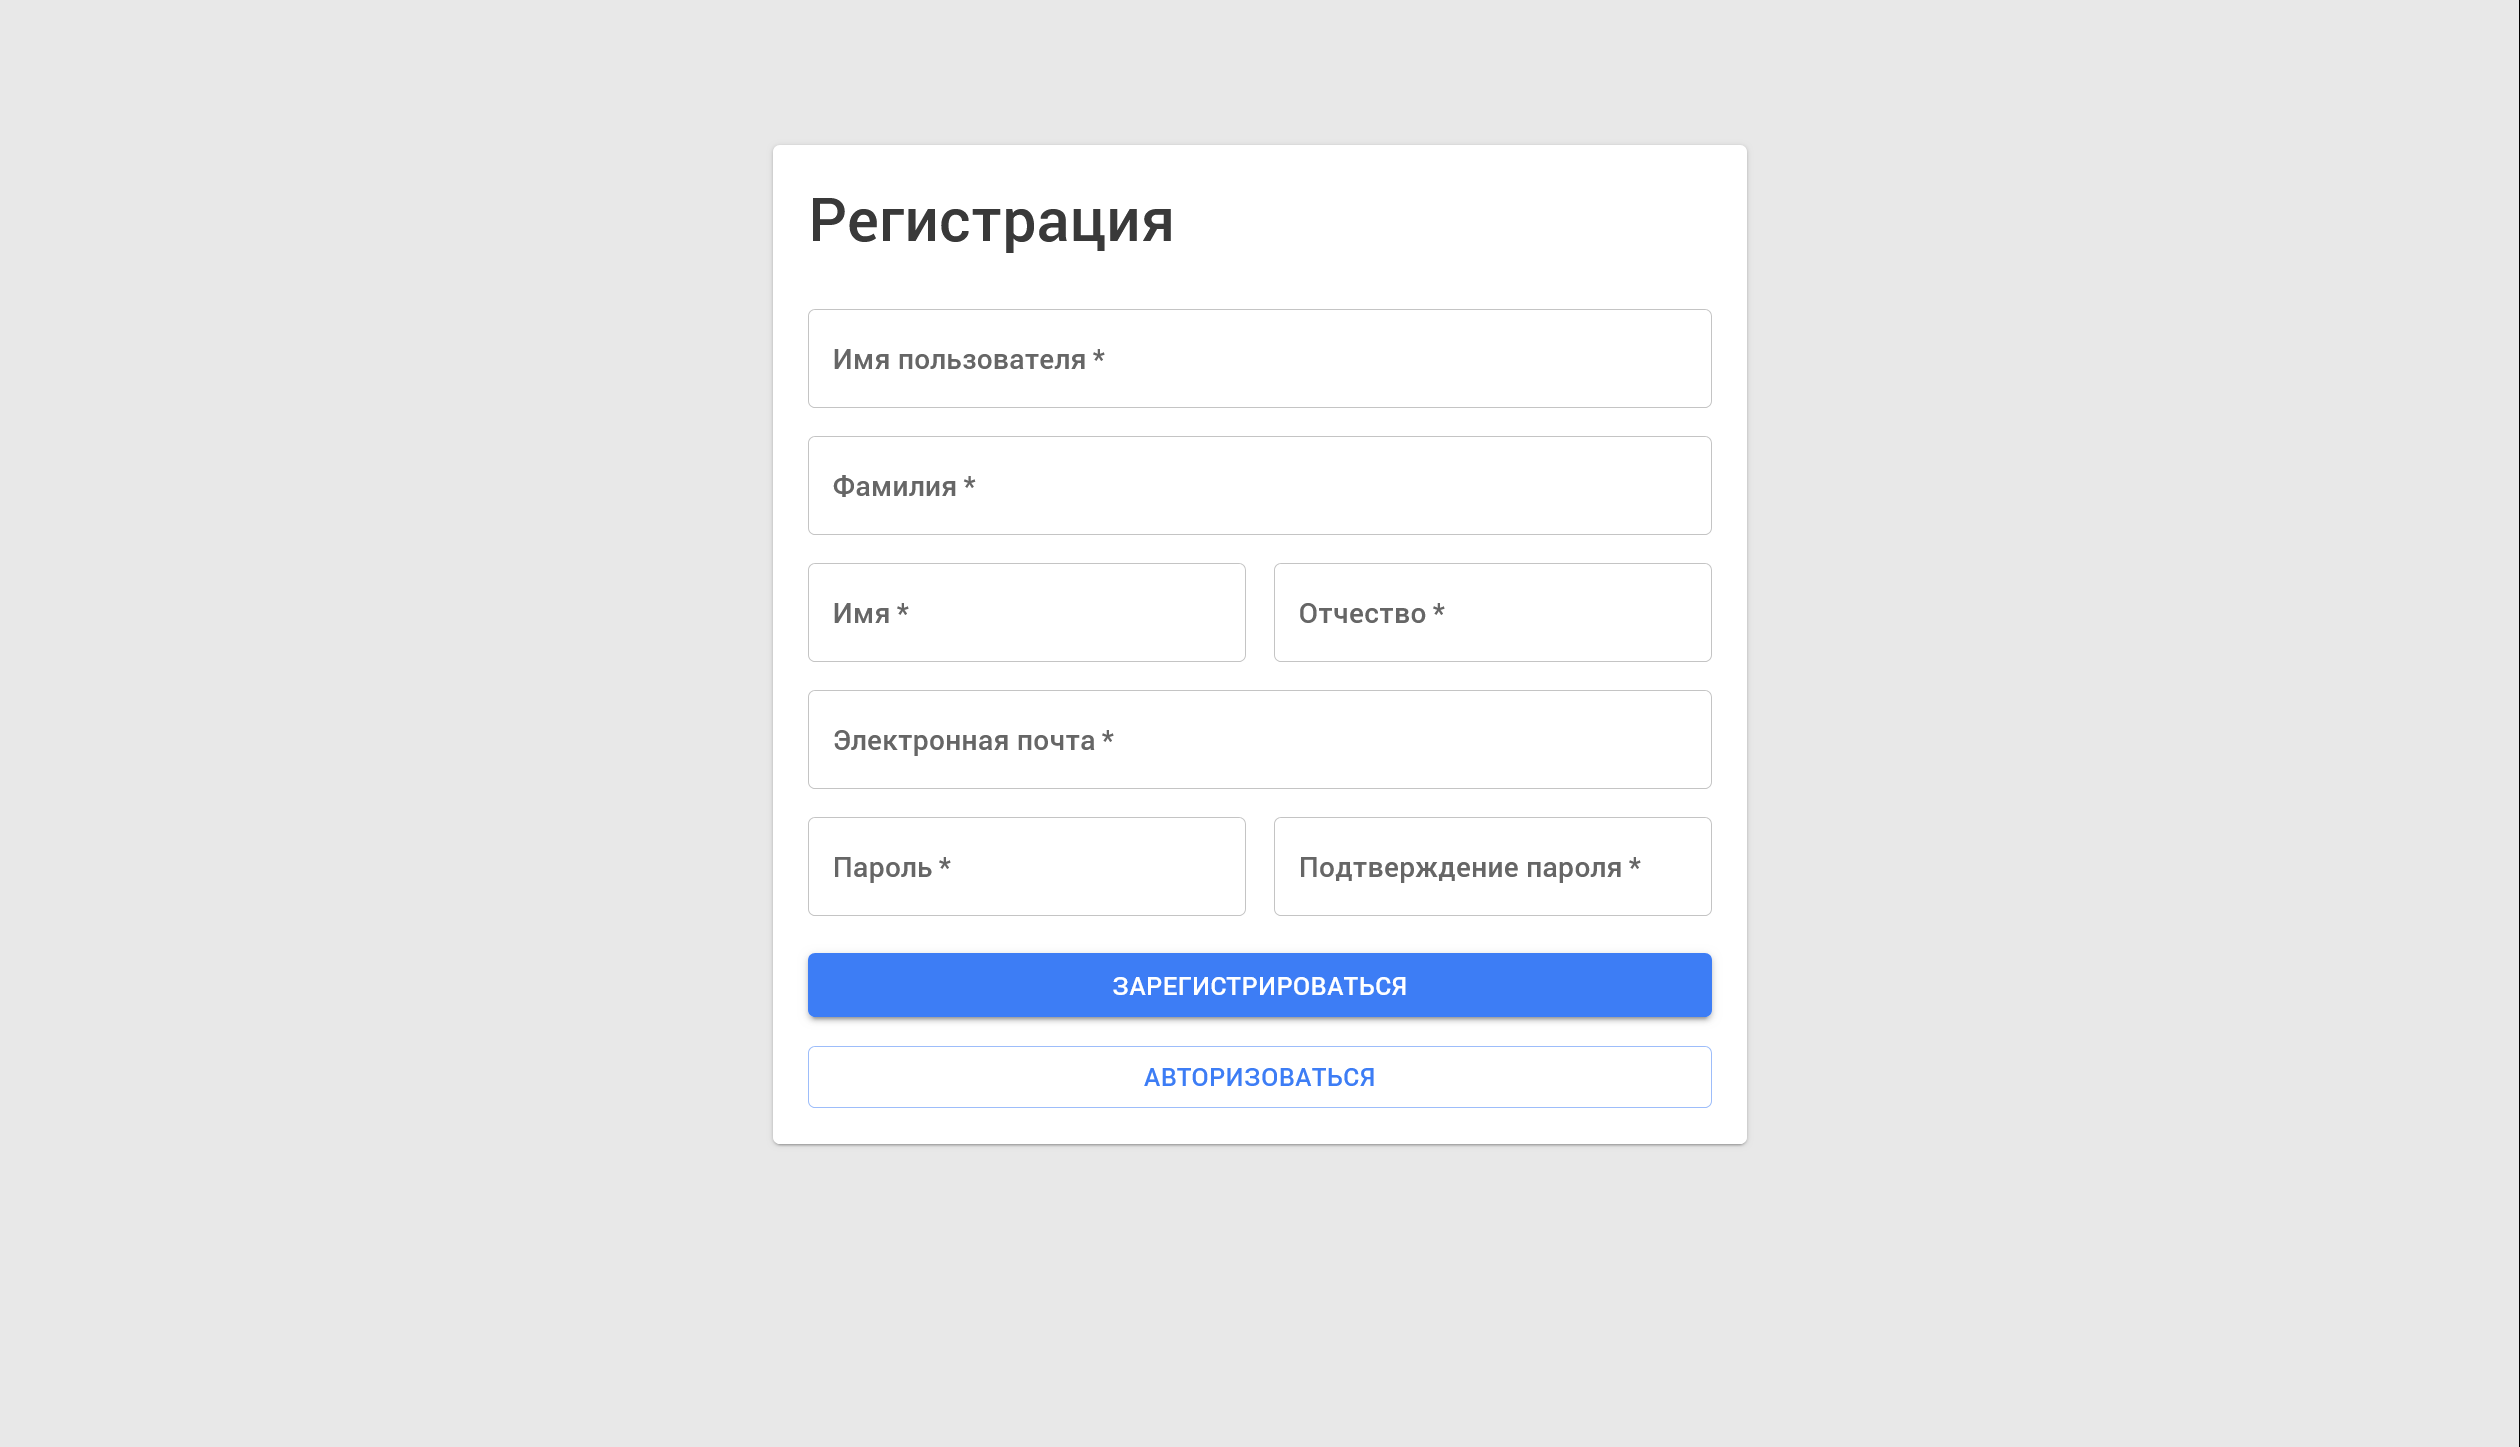
\includegraphics[width=\textwidth]{images/screenshots/doctor_registration}
    \caption{Аутентификация.}
    \label{fig:figure41}
\end{figure}


\subsection{Главная страница}\label{subsec:-2}
На главной странице уже появляется хэдер, который есть во всем приложении, кроме страницы аутентификации и регистрации врача.
(См.\ рис. \ref{fig:figure5})
В нем есть ссылки на саму главную страницу, на страницу регистрации пациента, так же имя врача, ссылка на его персональную страницу и возможность выхода из аккаунта.
В основном окне представлена таблица с результатами последних опросов, которые прошли пациенты.
В каждой строке нам важно знать, в какое время это произошло, с кем конкретно.
Важная графа с оценкой результатов опроса, она меняет свой цвет в зависимости от результата, чтобы врач мог сразу выделить отрицательные результаты и приступать к дальнейшим действиям.
Есть статус просмотрено у каждого опроса, который меняется нажатием иконки.
\begin{figure}[ht]
    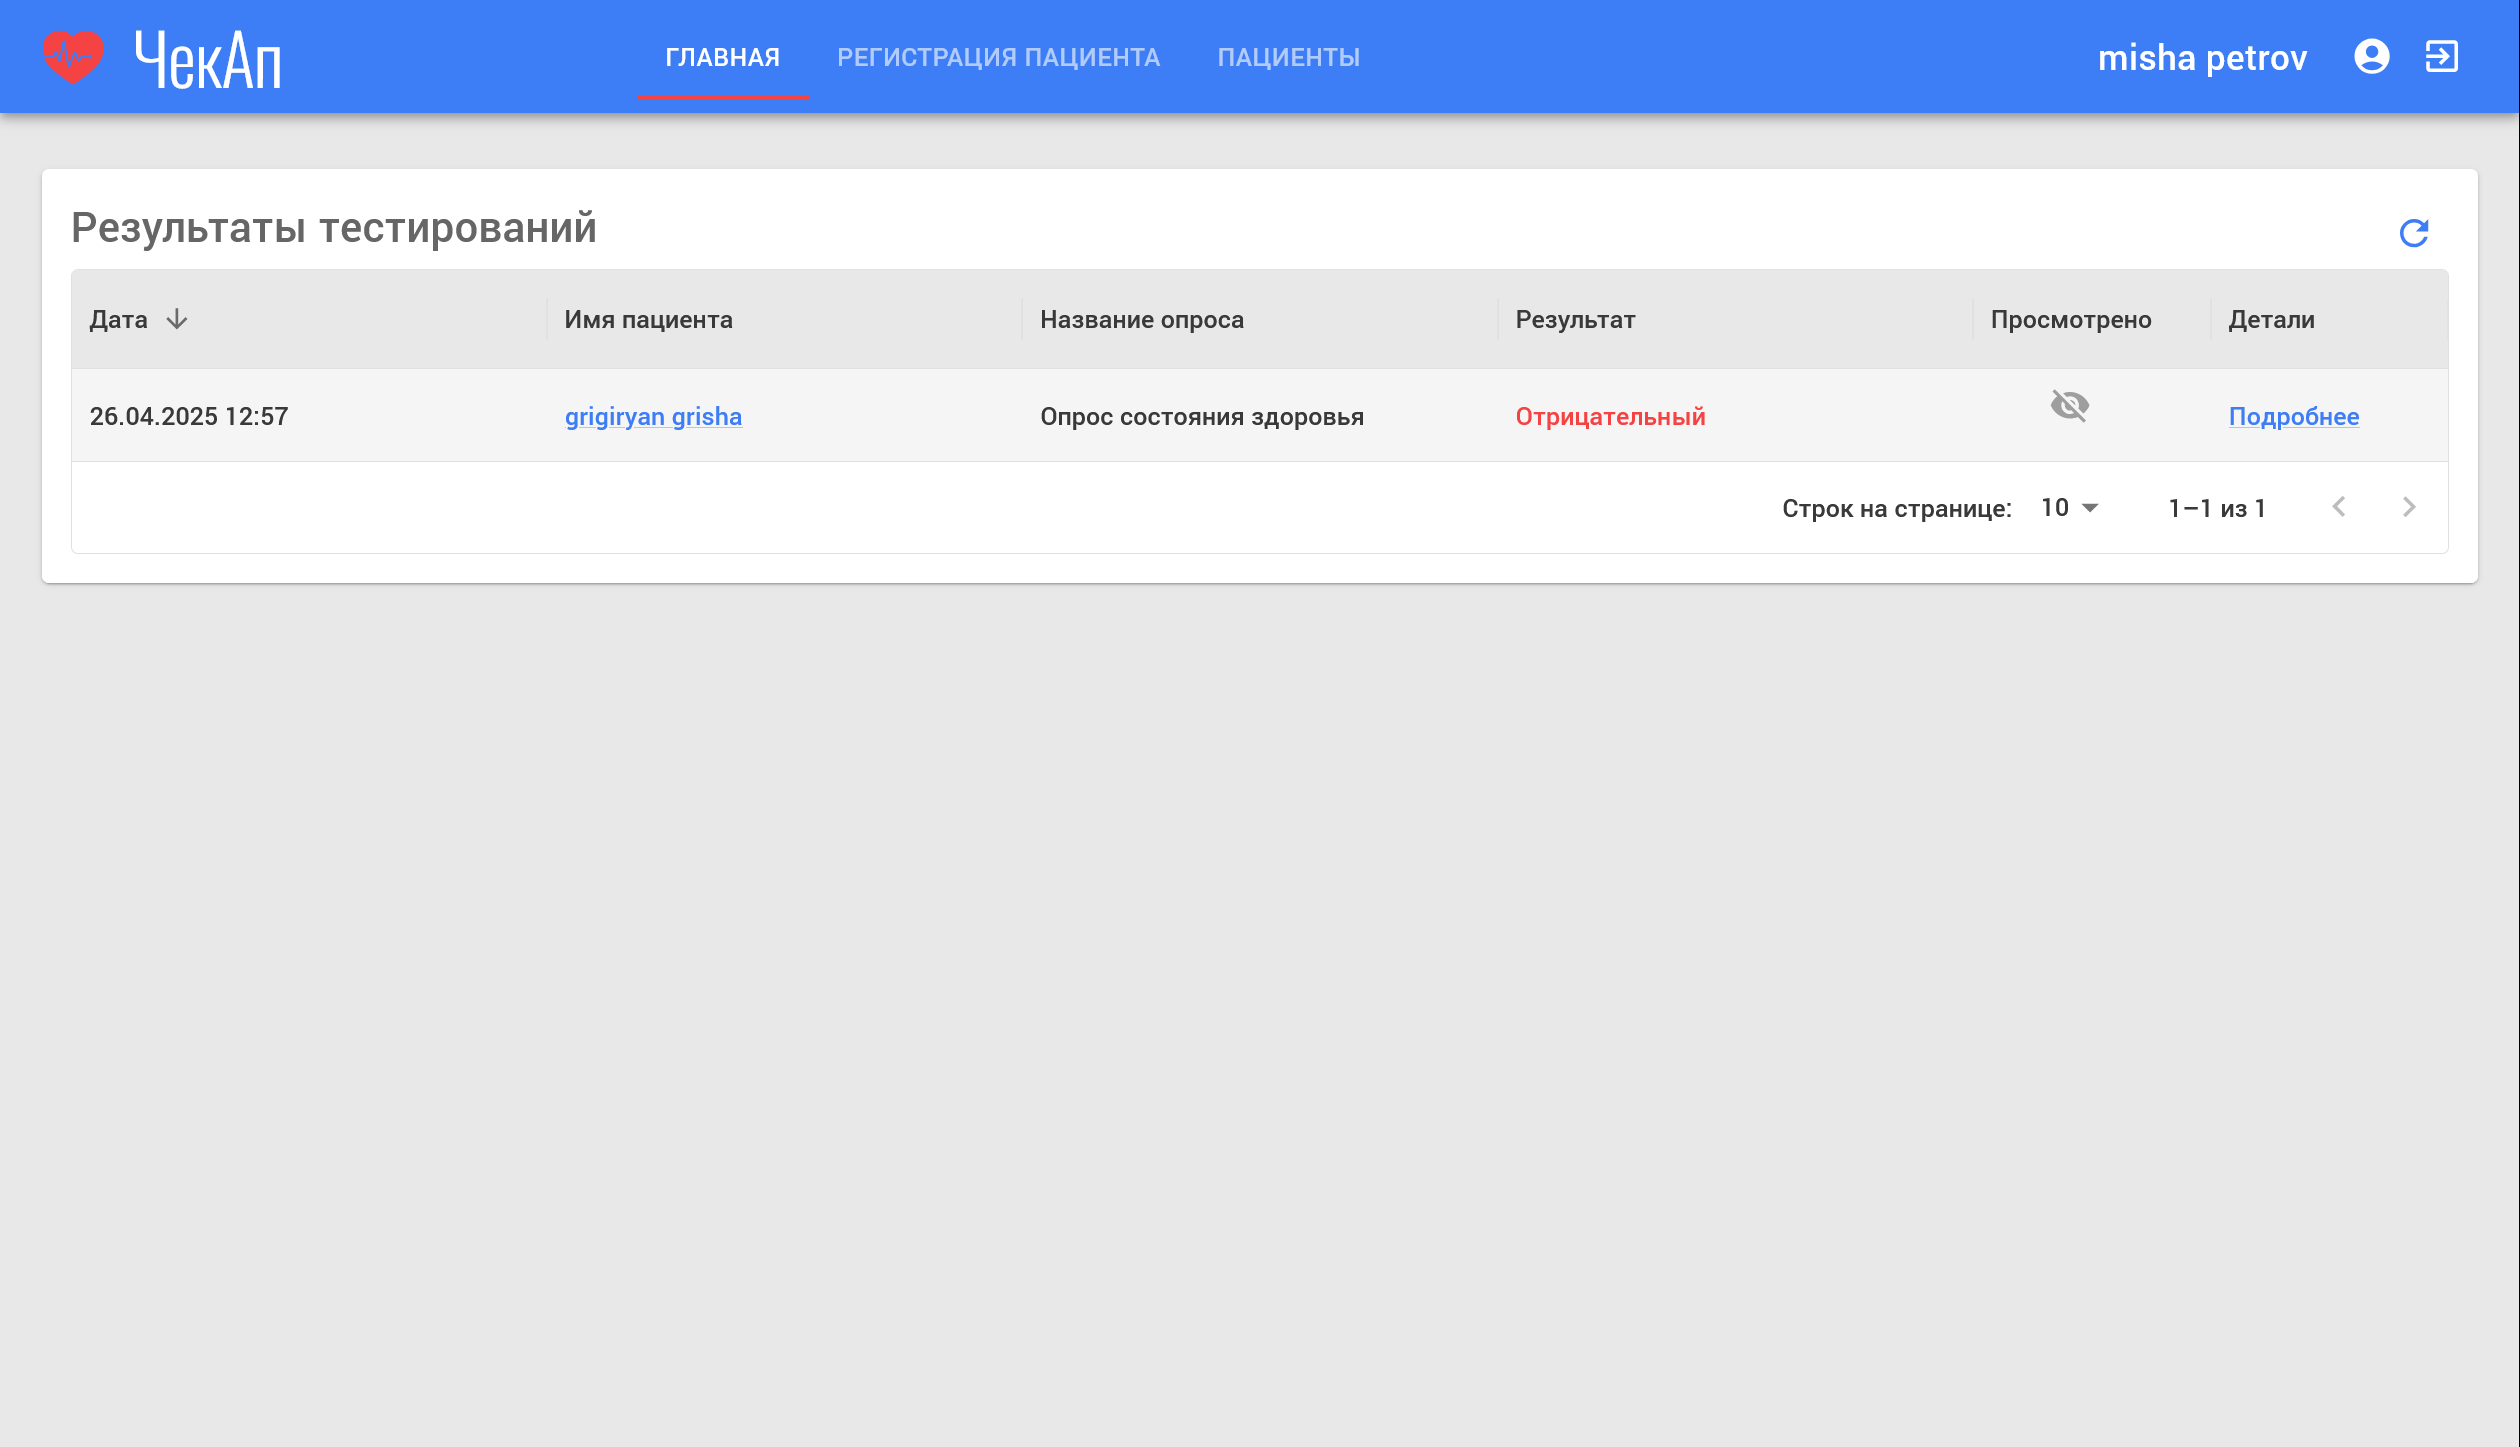
\includegraphics[width=\textwidth]{images/screenshots/main_page}
    \caption{Главная страница.}
    \label{fig:figure5}
\end{figure}

\subsection{Пациенты}\label{subsec:-22}
На данной странице представлены все пациенты, которые принадлежат данному врачу.
(См.\ рис. \ref{fig:figure51})
Их можно отсортировать по имени, произвести поиск по частям имени, перейти на страницу пациента.
\begin{figure}[ht]
    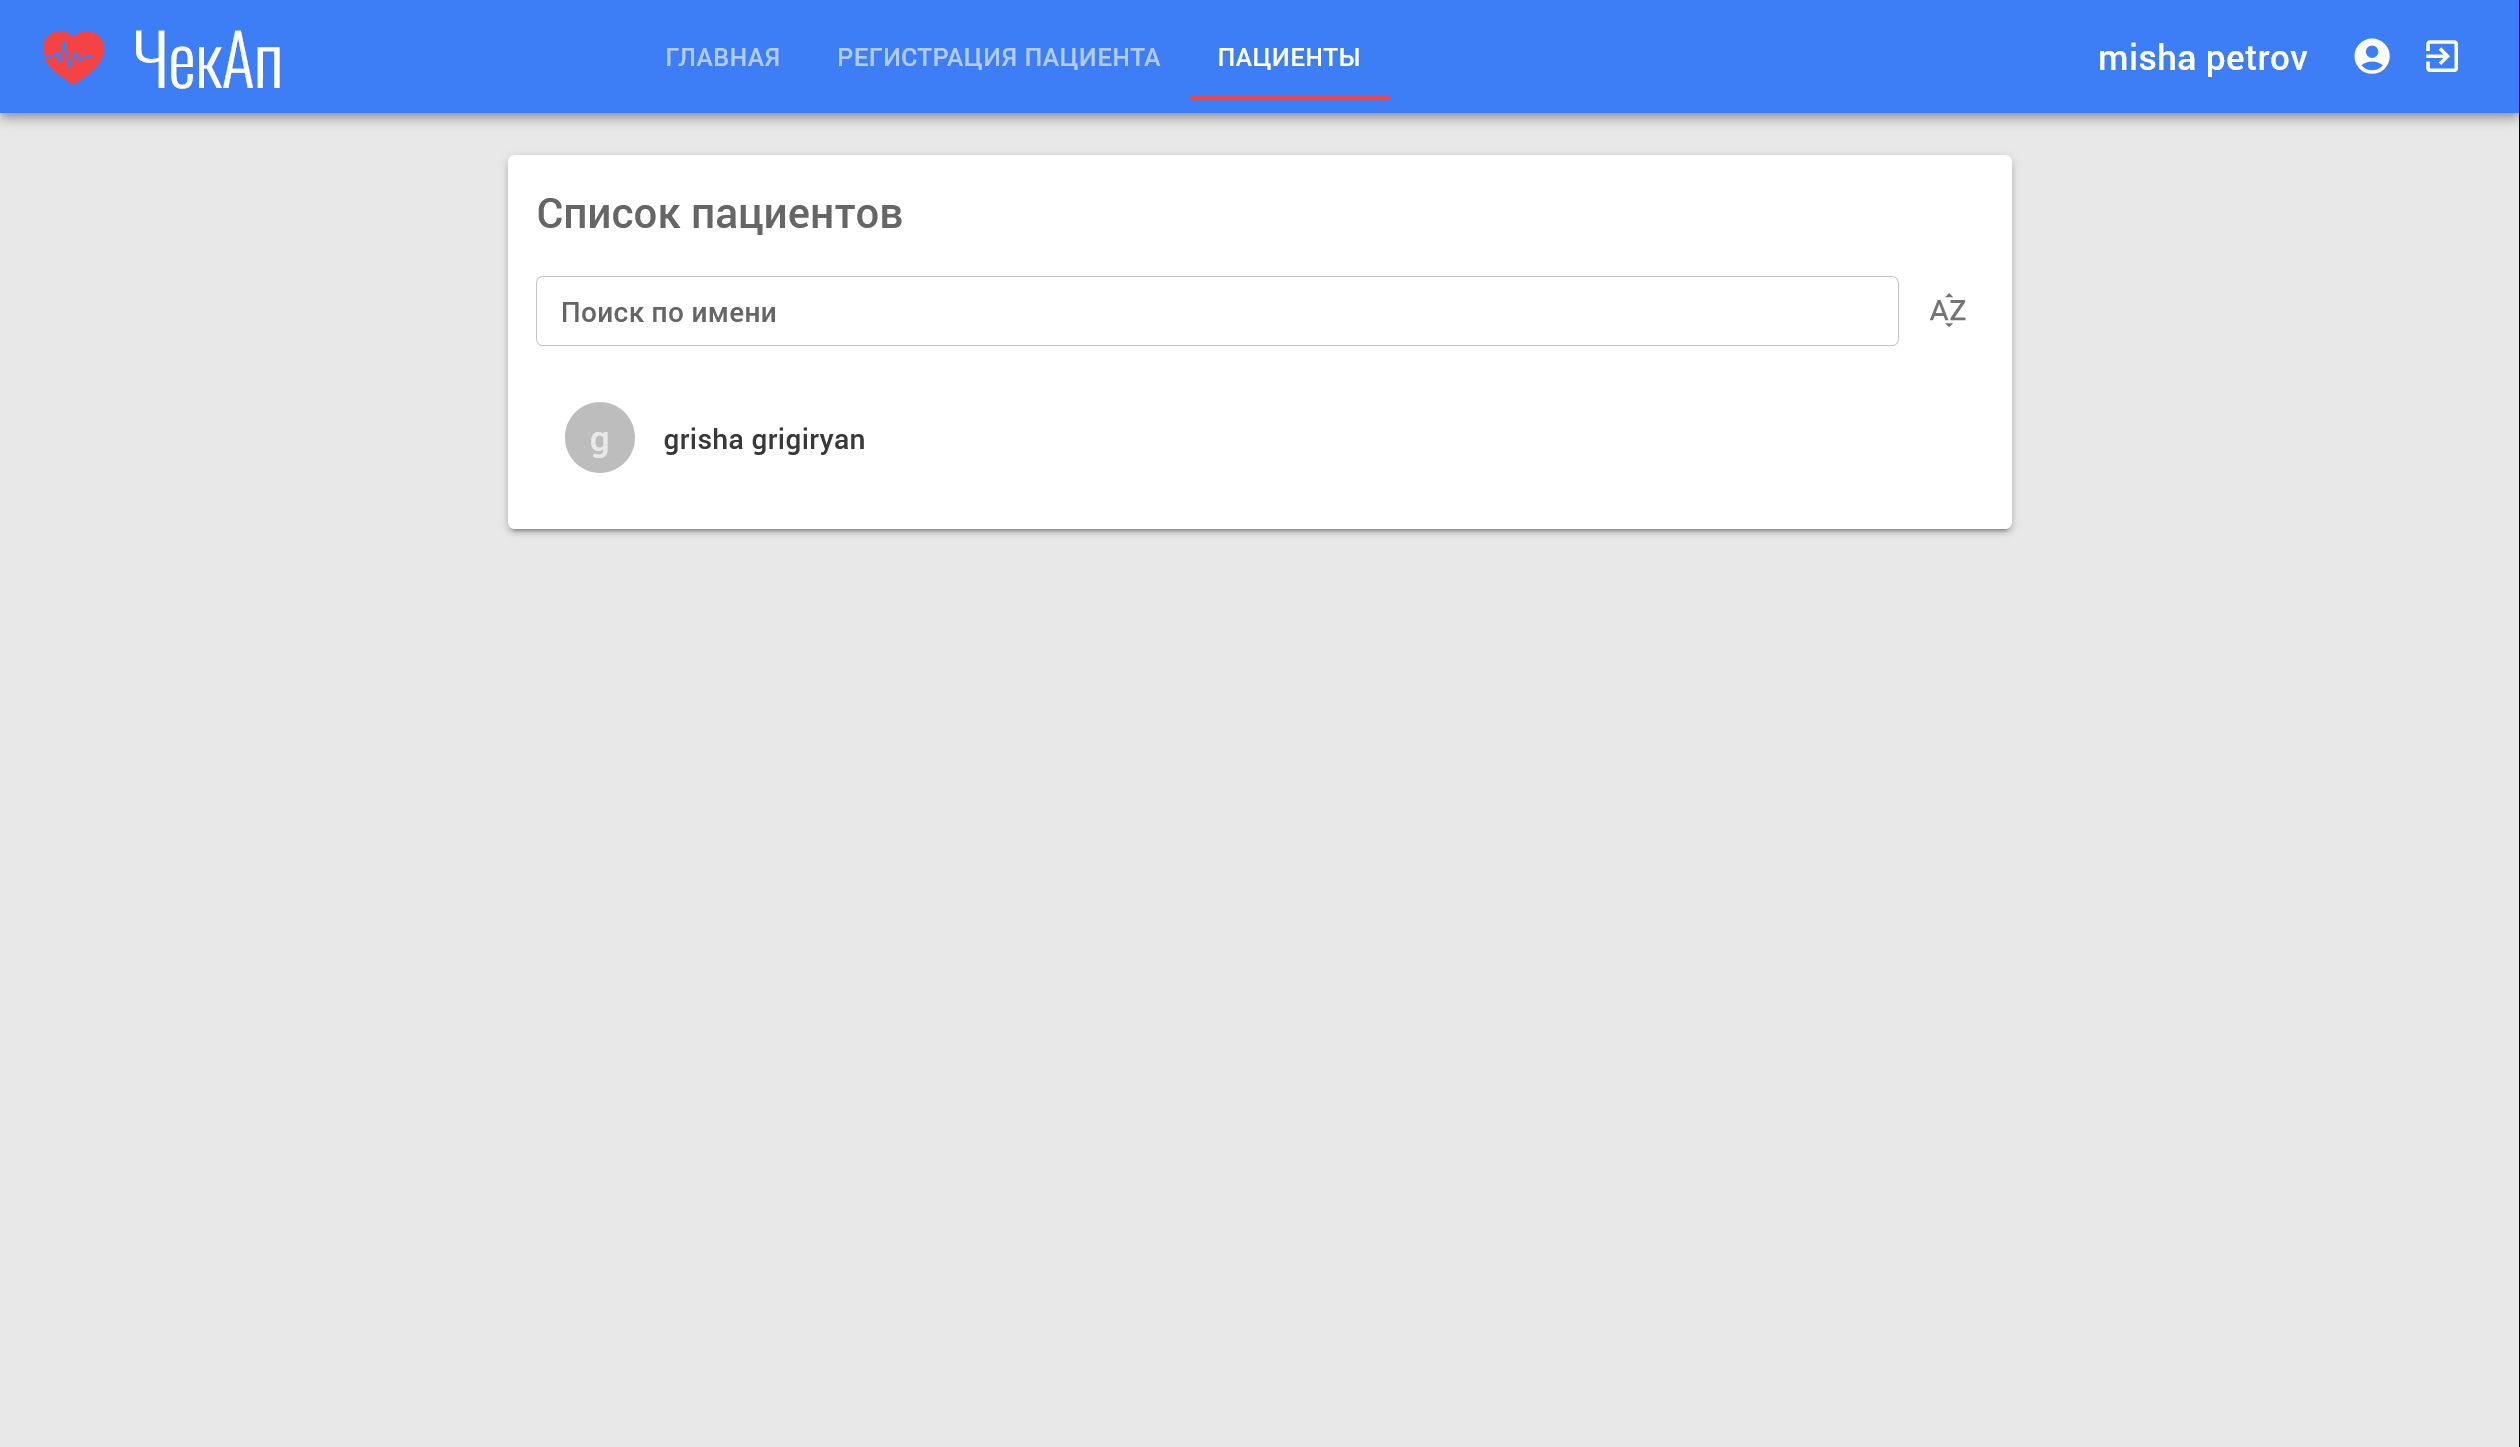
\includegraphics[width=\textwidth]{images/screenshots/patients}
    \caption{Пациенты.}
    \label{fig:figure51}
\end{figure}


\subsection{Пациент}\label{subsec:-222}
На данной странице представлены данные пациента: ФИО, телефон, электронная почта, его фотография (при наличии).
Рядом с номером телефона есть кнопка копирования номера пациента, если открывать с мобильного устройства, то так же будет предложение сразу открыть его в приложении для звонков.
(См.\ рис. \ref{fig:figure52})
Представлена статистика опросов.
Это таблица.
Каждый столбец соответствует одному дню, вверху подписаны число и месяц.
Каждый квадратик соответствует одному опросу, в зависимости от статуса опроса он меняет цвет.
Чтобы узнать чуть подробнее можно навести на него.
(См.\ рис. \ref{fig:figure521})
Там написаны детально: дата, статус и название опроса.
Чтобы узнать подробно об опросе, нужно нажать на квадратик.

\begin{figure}[ht]
    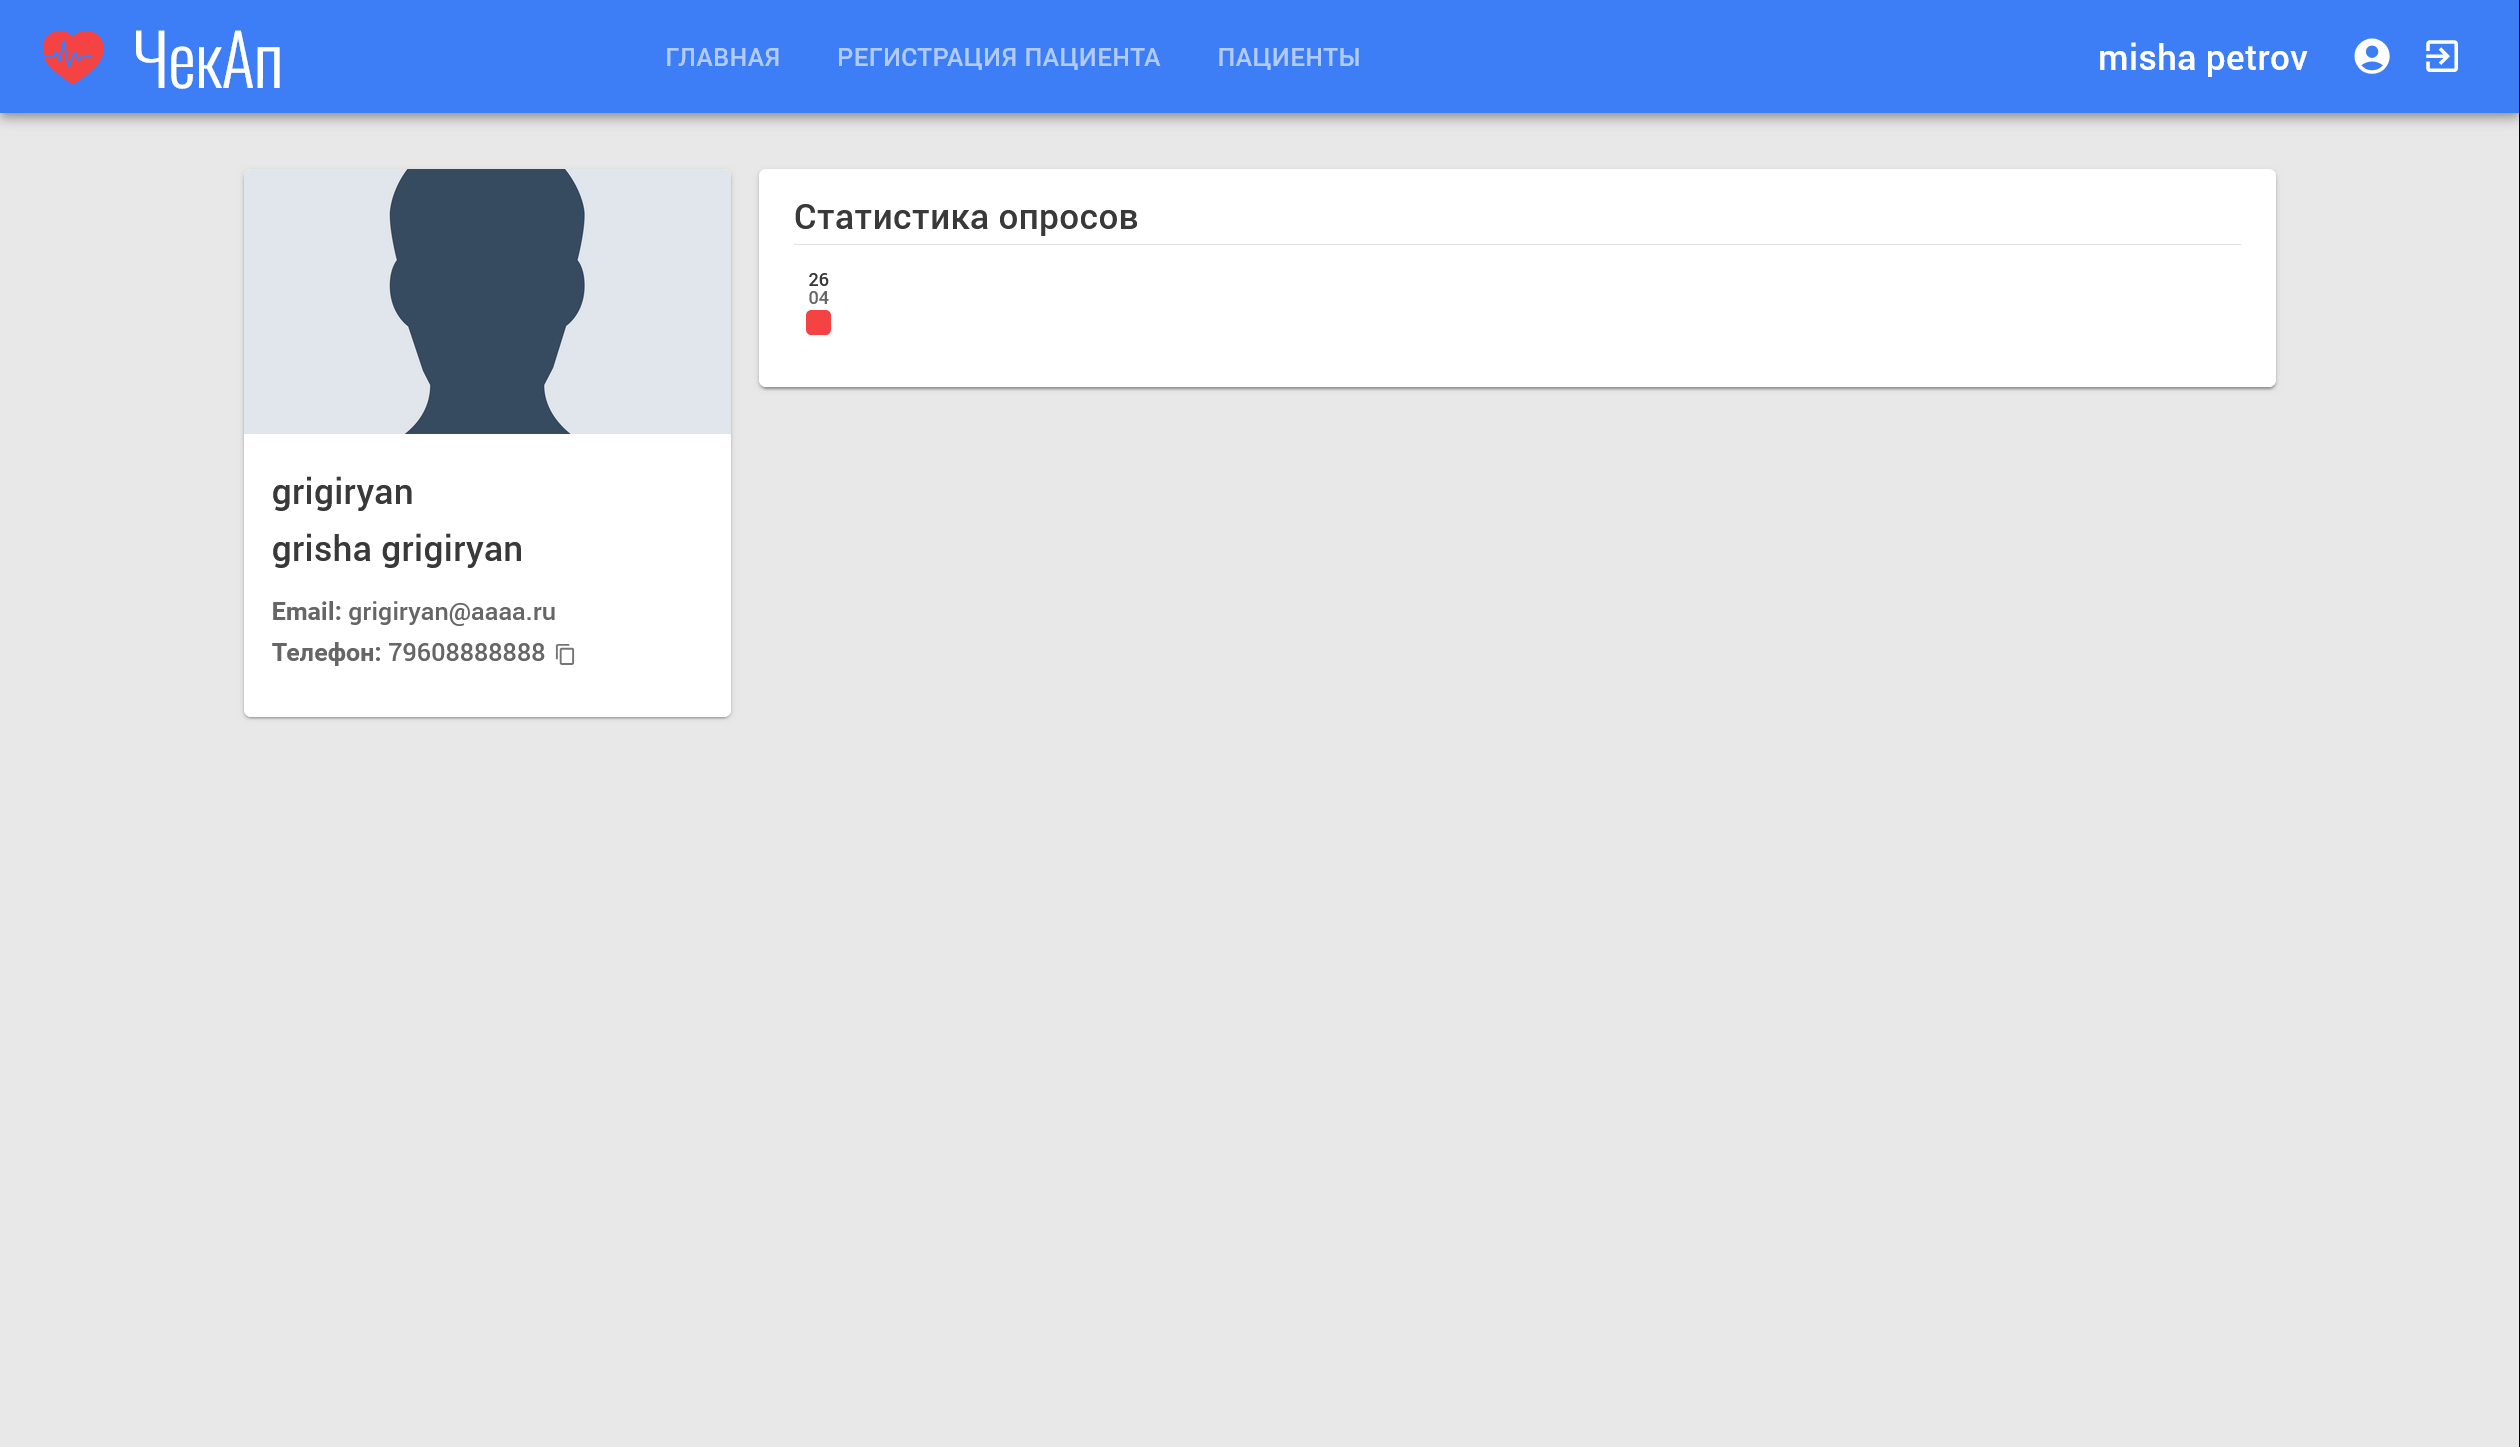
\includegraphics[width=\textwidth]{images/screenshots/patient}
    \caption{Пациенты.}
    \label{fig:figure52}
\end{figure}

\begin{figure}[ht]
    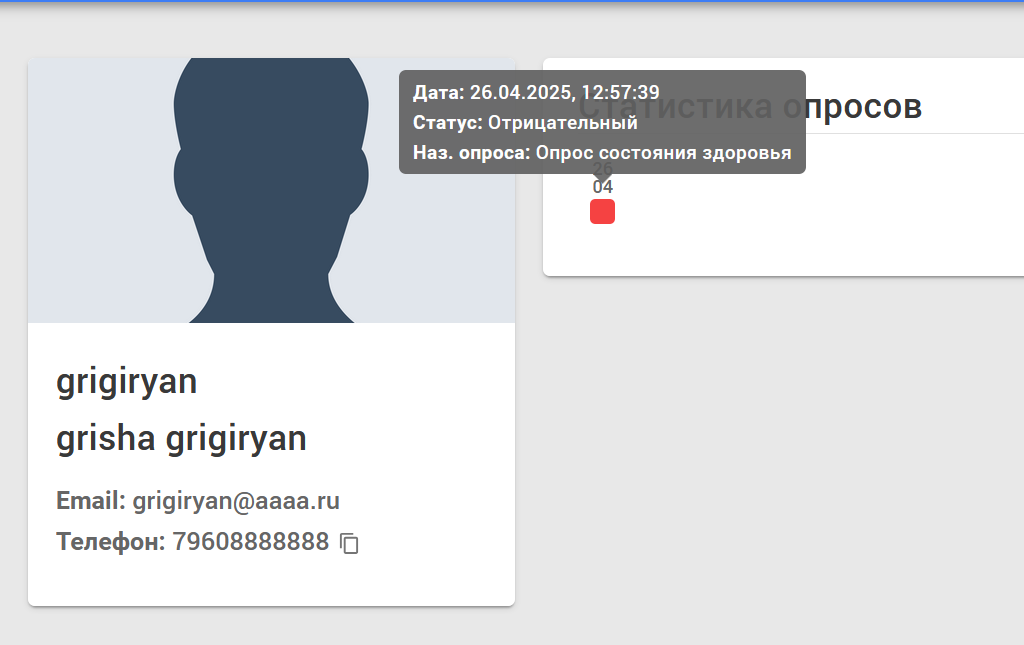
\includegraphics[width=\textwidth]{images/screenshots/patient_hover}
    \caption{Поведение таблицы опросов пациента при наведении на квадрат.}
    \label{fig:figure521}
\end{figure}


\subsection{Опрос}\label{subsec:2}
На страницу с конкретным прошедшим опросом можно перейти по ссылке из главной страницы или страницы пациента.
Здесь представлено подробно о пациенте аналогично странице пациента.
(См.\ рис. \ref{fig:figure6})

Та же представлены конкретные вопросы и ответы для большей возможности оценки ответов лично врачом.
Есть название опроса и его порядковый номер среди подобных опросов у этого пациента.
\begin{figure}[ht]
    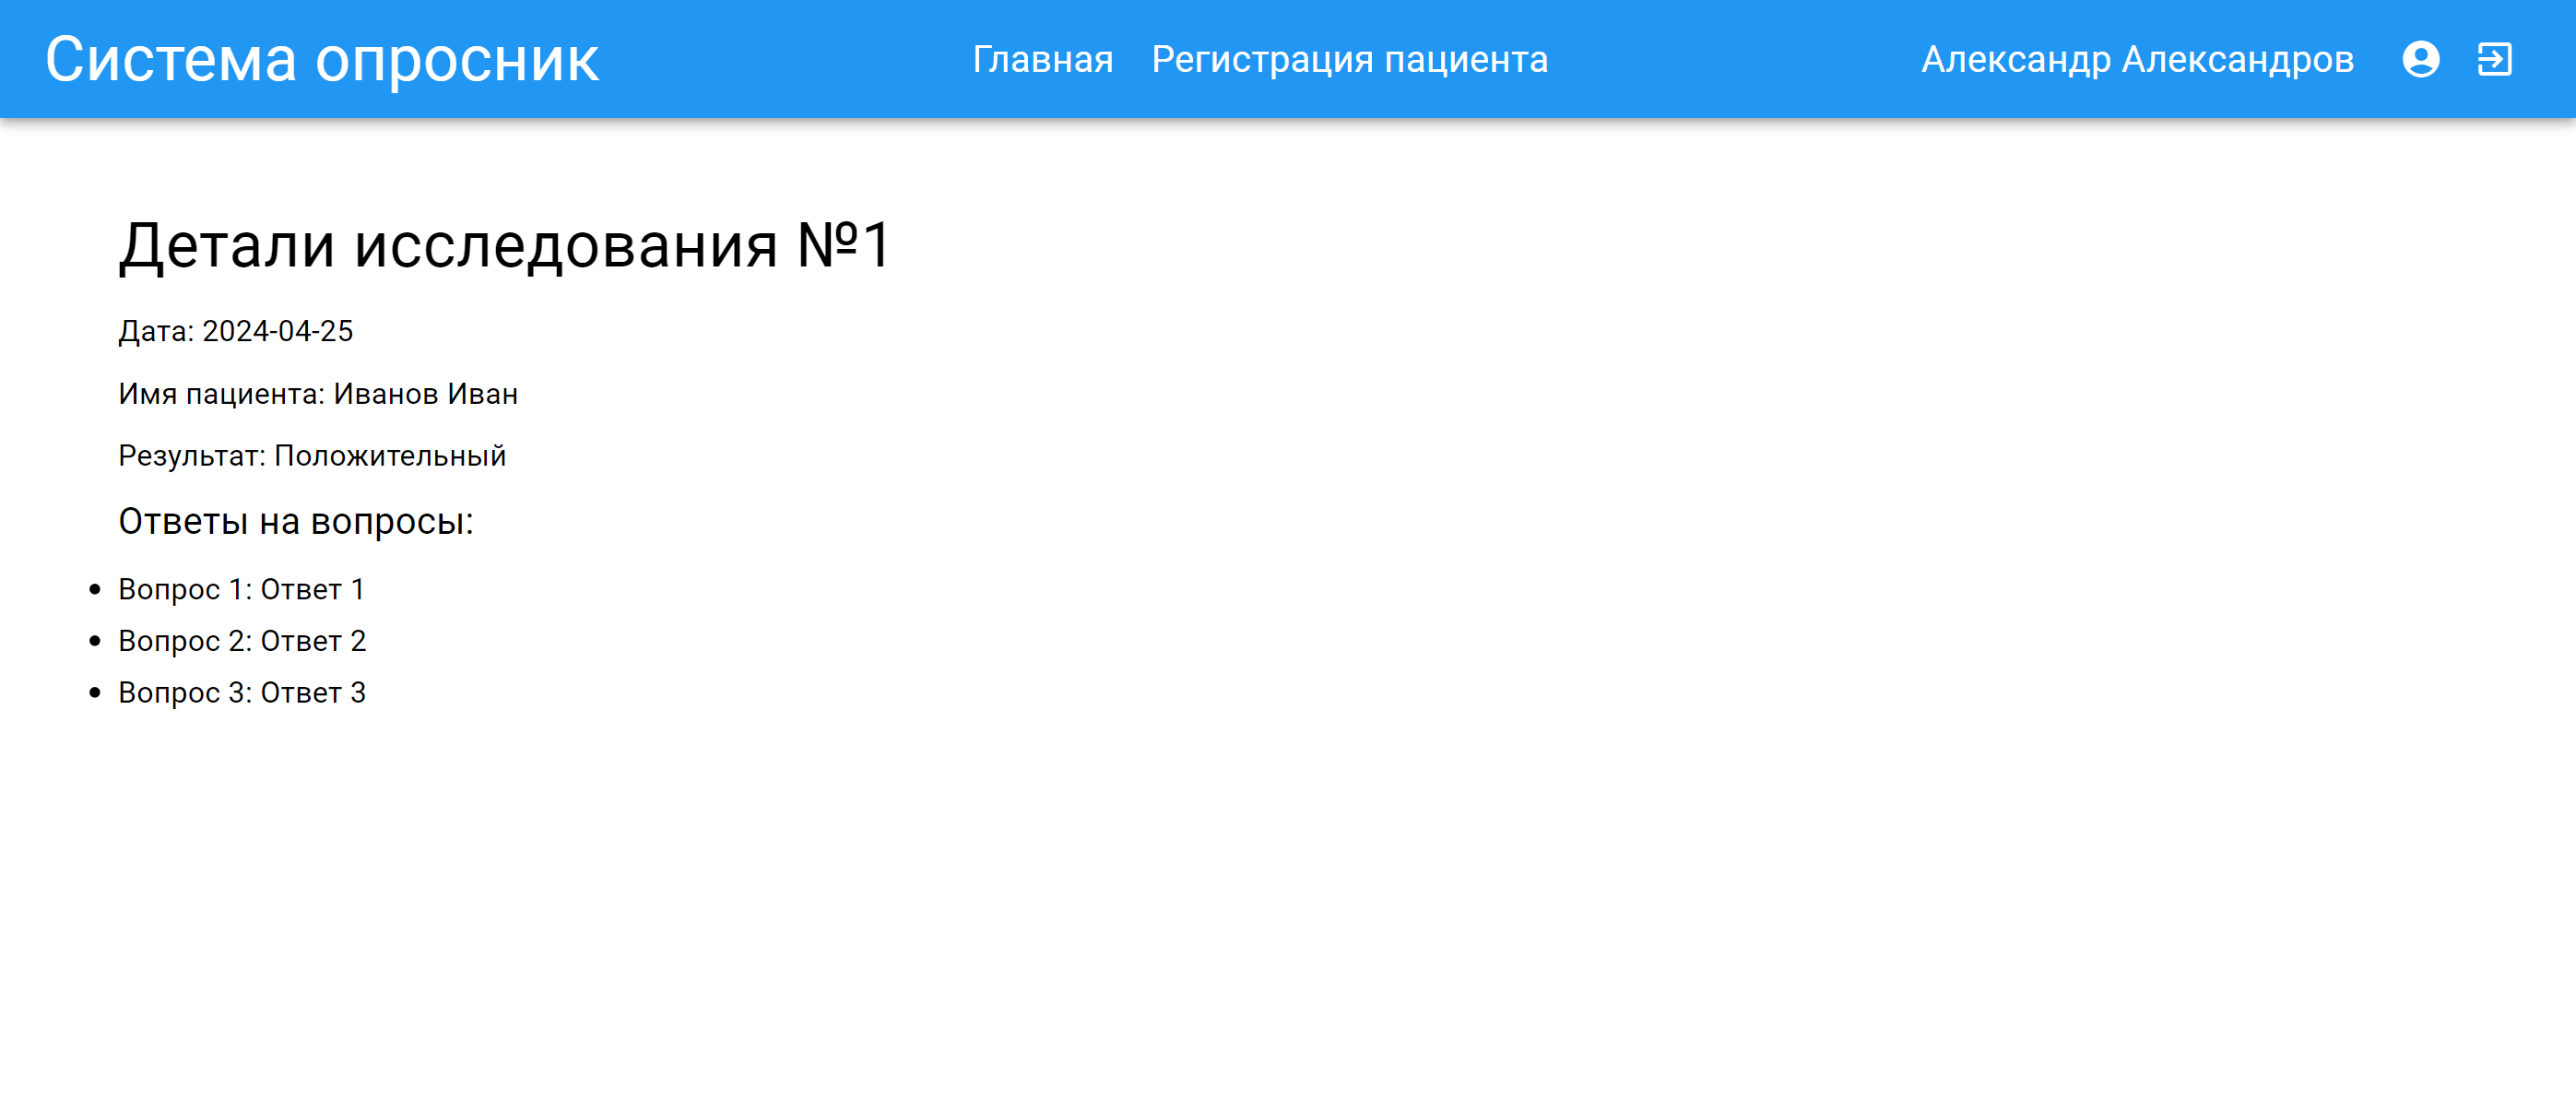
\includegraphics[width=\textwidth]{images/screenshots/inquirer}
    \caption{Страница опроса пациента.}
    \label{fig:figure6}
\end{figure}

\newpage
\subsection{Регистрация пациента}\label{subsec:-3}
На этой странице представлена форма для регистрации нового пациента (См.\ рис~\ref{fig:figure7})
\begin{figure}[ht]
    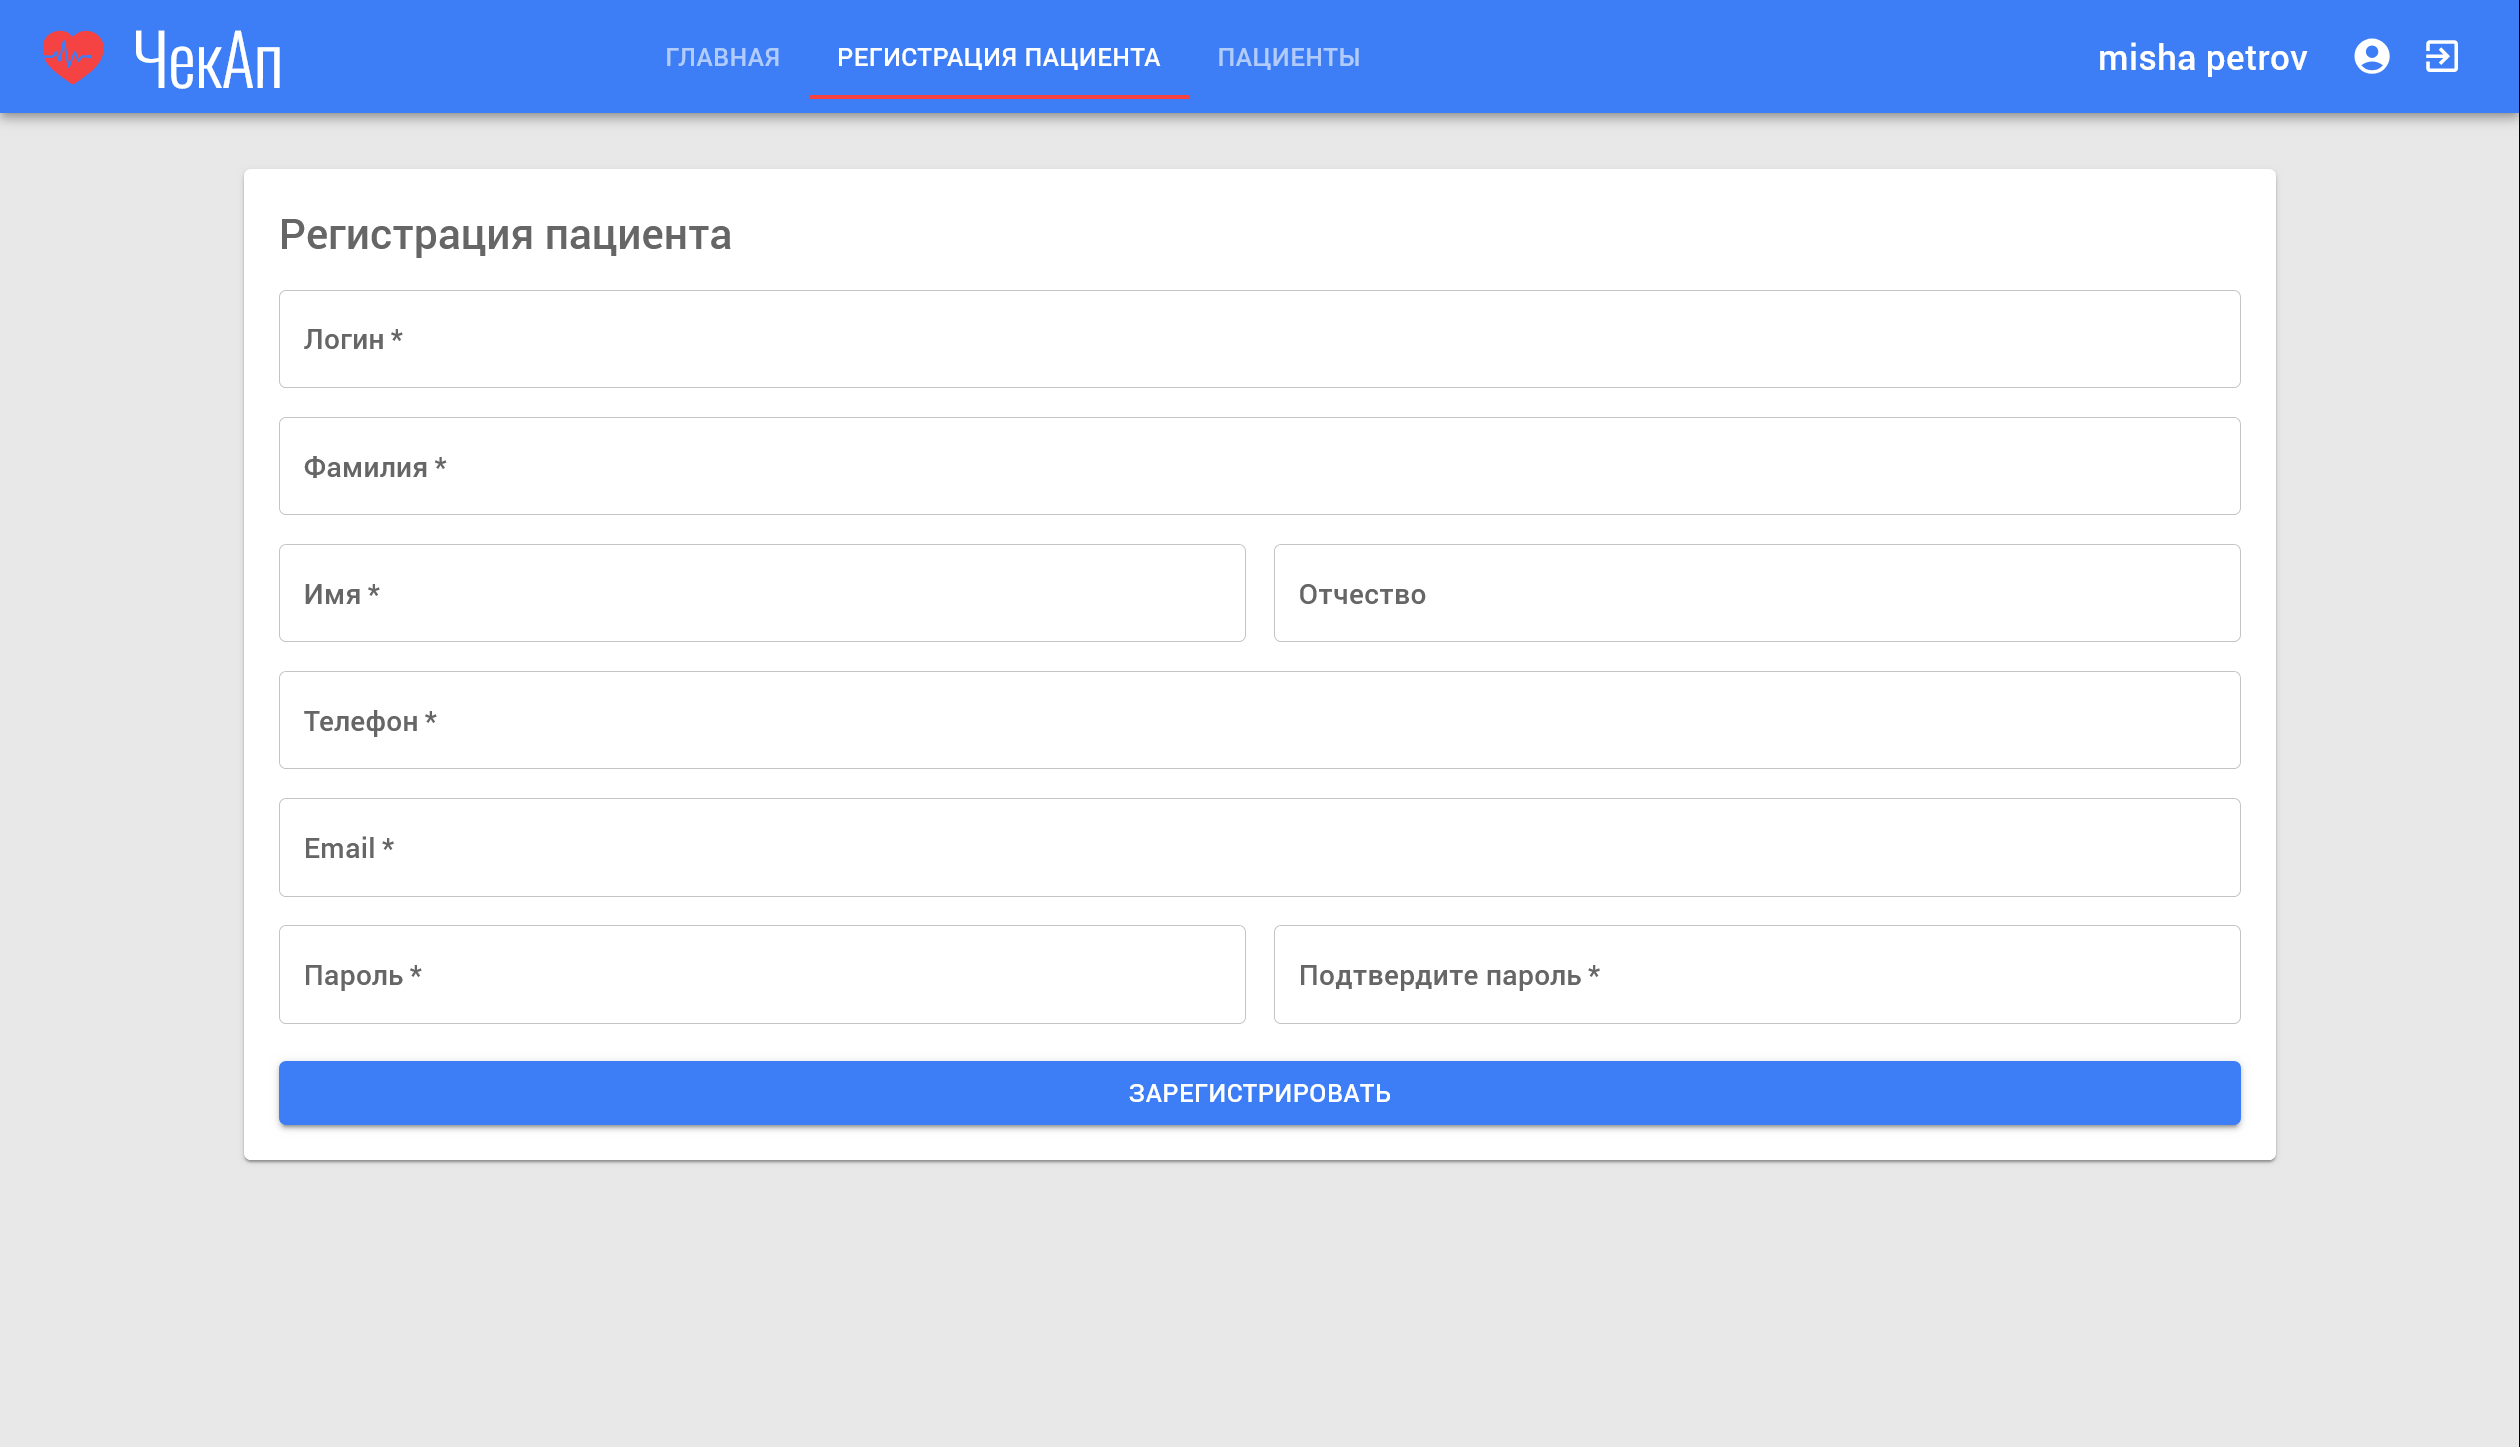
\includegraphics[scale=0.17]{images/screenshots/patient_registration}
    \caption{Форма регистрации пациента.}\label{fig:figure7}
\end{figure}